\section{Введение}

\subsection{О приближениях}

    Математический анализ "--- это наука о приближениях.

    \begin{definition}
        Определение производной по Коши:
        Пусть $f = f(x)$ -- функция, число $A$ называется производной функции $f$ в
        точке $x$, если при неограниченным уменьшении $|h|$ \[
        P(\varepsilon, \delta) :=   0 < |h| < \delta \longrightarrow \left(\frac{f(x + h) - f(x)}{h} - A\right) < \varepsilon,
        \text{ где } P(x) = \text{истина или ложь} \]
        \[\forall \varepsilon > 0 \
        \exists \delta > 0 \ P(\varepsilon, \delta)
        \]
    \end{definition}
    \begin{example}
        $f(x) = x^2$:
        \begin{equation*}
            \frac{f(x + h) - f(x)}{h} = \frac{x^2 + 2xh + h^2 - x^2}{h} = 2x + h 
        \end{equation*}
        Проверим, что $A  = 2x$ является производной $f$ в точке $x$:
        \begin{equation*}
            \forall \varepsilon \ \exists \delta > 0 \ (0 < |h| < \delta) \rightarrow \left|\frac{(f(x + h )
            - f(x))}{h} - 2x\right| < \varepsilon
        \end{equation*}
        Дано $\varepsilon > 0$. Какое $\delta$ взять, чтобы $P(\varepsilon, \delta) = 1$?
        Если взять $\delta = \dfrac{\varepsilon}{2}$, то $0 < |h| < \delta \longleftrightarrow  |h|\hm{<} \dfrac{\varepsilon}{2}
        \longrightarrow P(\varepsilon, \delta) = 1$
    \end{example}
    \begin{exercise}
        Проверить, что утверждения имеют одинаковые значения: (кто не с нами, тот 
        против нас) $\longleftrightarrow$ (кто не против нас, тот с нами)
    \end{exercise}
    В этом семестре:
    \begin{enumerate}
        \item приближение функций многочленами
        \item евклидова топология вещественной прямой
        \item приложения к исследованию функций
    \end{enumerate}
    \subsection{Кванторы}
    \begin{enumerate}
        \item  $\forall x \ P(x)$ --- для любого $x$ выполненоолнено $P(x)$ 
        \item $\exists x \ P(x) $ --- существует $x$, для которого выполненоолнено $P(x)$ 
        \item $\exists ! x \ P(x) $ --- существует и единственно $x$,
        для которого выполненоолнено $P(x)$ 
         
    \end{enumerate}
    \begin{equation*}
        \exists ! x \ P(x)  = \exists x(P(x)) \land (\forall y \ P(y) \lra y = x)
    \end{equation*}
    \begin{equation*}
        \forall y (\forall x \ P(x, y))\longleftrightarrow \forall y, x \ P(x, y)
    \end{equation*}
    \subsubsection*{Порядок кванторов}
    \begin{enumerate}
        \item $\forall x\ \forall y\ P(x, y)$
        \item $\exists x\ \forall y\ P(x, y) $
        \item $ \forall x\ \exists y\ P(x, y) $
        \item $\exists x \ \exists y \ P(x, y) $
    \end{enumerate}
    \begin{note} 
        Важен ли порядок кванторов?
        \begin{equation*}
            \forall x \in \R\ \exists n \in \N \ n > x \ \text{--- истина}
        \end{equation*}
        \begin{equation*}
            \exists n \in \N \ \forall x \in \R \ x > n \ \text{--- ложь}
        \end{equation*}
    \end{note}
\subsection{Некотрые сведения из теории множеств}
    \begin{definition}
        Пусть $X$ и $Y$ --- множества, тогда множество, состоящее из всех возможных пар $(x, y)$,
         где $x \in X,\ y \in Y$ называется декартовым произведением $X$ и $Y$ и обозначается
        $X\times Y$. 
    \end{definition}
    \begin{note}
        Пишут: \begin{equation*}
            X \times Y := \{(x, y)|\ x \in X,\ y \in\ Y \} 
        \end{equation*}
    \end{note}
    \begin{note}
        \begin{equation*}
            X^2 := X \times X
        \end{equation*}
    \end{note}
    \begin{definition}
        Пусть $X$ -- множество. \begin{equation*}
            2^X : = \{ Y | Y \subset X\}
        \end{equation*}
    \end{definition}
    \begin{note}
        Здесь \begin{equation*}
            Y \subset X \xleftrightarrow{\triangle} \forall y \ \left(
                y \in Y \longrightarrow y \in X
            \right)
        \end{equation*}
        \begin{reminder}
            \begin{equation*}
                \xleftrightarrow{\triangle} \text{---  по определнию}
            \end{equation*}
        \end{reminder}
    \end{note}
    \begin{proposition}
        Если $ X $ состоит из $ n $ элементов, то $ 2^X $ состоит из $ 2^n $ 
        элементов.
    \end{proposition}
    \begin{definition}
        Отношением на множестве $ X $ называется $ \forall  $ подмножества
        $ R\subset X^2 $, при этом $ \forall x, y \in X $: \begin{equation}
            x \text{ и } y \text{ находятся в отношении } R \Longleftrightarrow
            (x, y) \in R \xleftrightarrow{\triangle} xRy
        \end{equation}
    \end{definition}
    \begin{example}
        Пусть $ R \subset X^2 $, $ x,y \in X $, тогда если $ (x, y) \in R $,
        то $ xRy $, иначе $ x $ и $ y $ не состоят в отношении $ R $. 
    \end{example}
    \begin{definition}
        Пусть $ X, Y $ -- множества, $ \Gamma\subset X  \times  Y$, причём $ \forall x \in X \exists 
        !\ y \in  Y: (x, y) \in \Gamma $. Тогда тройкой $ f : = \left(X, Y, \Gamma\right) $ называется
        функцией, а $ \Gamma $ --- её графиком.
    \end{definition}
    \begin{note}
        При этом \begin{equation}
            (y = f(x)) \xleftrightarrow{\triangle}\left(x \in X \land y \in Y\, \land 
            (x, y) \in \Gamma\right)
        \end{equation}
    
    \begin{figure}
        \centering
        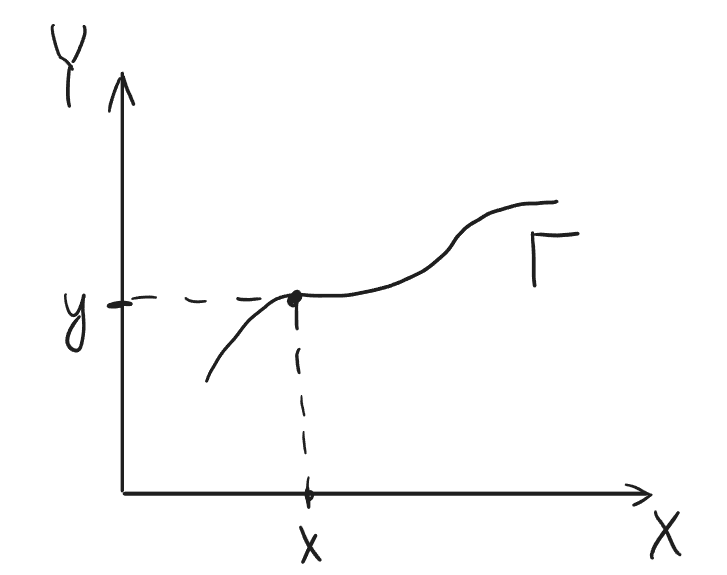
\includegraphics[width = 0.3\textwidth]{image1.png}
    \end{figure}
    
        Пишут: \begin{enumerate}
            \item $ f:  X \to  Y $
            \item $ f: X\mapsto f(x) $ \begin{example}
                $ f: n \mapsto n^2 $
            \end{example}
            \item $ f: X \ni x \mapsto f(x) \in Y $
        \end{enumerate}
    
        Если $ f: X \times Y \to Z $, то $ \forall x \in  X, \forall y \in  
        Y $ вместо $ f((x, y)) $ пишут $ f(x, y) $.
    \end{note}
   